% =====================================================================
%  The Medium Vertex and the Direction of a Protein Process
%
%  Gives a semantics to the medium vertex m, which the Shakespeare
%  specification declares and never uses. Three consequences follow:
%  solvent role becomes derivable, reaction direction becomes a property
%  of the medium rather than of the reaction, and the framework acquires
%  its first principled refusal.
% =====================================================================
\documentclass[11pt,twocolumn,a4paper]{article}

\usepackage[utf8]{inputenc}
\usepackage[T1]{fontenc}
\usepackage{lmodern}
\usepackage[a4paper,margin=2.4cm]{geometry}
\usepackage{amsmath,amssymb,amsthm,mathtools}
\usepackage{bm}
\usepackage{booktabs}
\usepackage{array}
\usepackage{enumitem}
\usepackage{microtype}
\usepackage{xcolor}
\usepackage{graphicx}
\usepackage{listings}
\usepackage[round,sort&compress]{natbib}
\usepackage[colorlinks=true,linkcolor=blue!45!black,
            citecolor=blue!45!black,urlcolor=blue!45!black]{hyperref}
\usepackage{cleveref}

% ---- Theorem-like environments ----
\newtheoremstyle{thmstyle}{\topsep}{\topsep}{\itshape}{}{\bfseries}{.}{.5em}{}
\theoremstyle{thmstyle}
\newtheorem{theorem}{Theorem}[section]
\newtheorem{lemma}[theorem]{Lemma}
\newtheorem{proposition}[theorem]{Proposition}
\newtheorem{corollary}[theorem]{Corollary}
\theoremstyle{definition}
\newtheorem{definition}[theorem]{Definition}
\newtheorem{rulename}[theorem]{Rule}
\newtheorem{principle}[theorem]{Principle}
\newtheorem{example}[theorem]{Example}
\theoremstyle{remark}
\newtheorem{remark}[theorem]{Remark}
\newtheorem{notation}[theorem]{Notation}

% ---- shakespeare listing style ----
\definecolor{shkw}{RGB}{30,64,175}
\definecolor{shcom}{RGB}{22,101,52}
\definecolor{shnum}{RGB}{180,83,9}
\definecolor{shstr}{RGB}{159,18,57}
\definecolor{shbg}{RGB}{250,250,250}
\lstdefinelanguage{shakespeare}{
  morekeywords={receiver,floor,cut,contact,close,complex,fold,track,until,
    yield,when,observe,catalyze,mutate,complete,where,in,as,let,medium,
    converge,diverge,with,by,reps,switch,import,module,ambient,depleted,
    export,assert,from,to,if,else,scene,perform,leaf,tree,role,emit},
  morekeywords=[2]{residue,cofactor,electronic,solvent,substrate,
    Atom,Contact,Complex,Path,Trajectory,Signature,Structure,Scalar,Cut,
    Medium,Role,structural,bulk,S,nu,thick,delta,valence,shape,vacancy,
    floorval,count,coherence,spin,orbital,depth},
  sensitive=true,
  morecomment=[l]{--},
  morestring=[b]",
  keywordstyle=\color{shkw}\bfseries,
  keywordstyle=[2]\color{shnum},
  commentstyle=\color{shcom}\itshape,
  stringstyle=\color{shstr},
  basicstyle=\ttfamily\small,
  backgroundcolor=\color{shbg},
  frame=single,framesep=4pt,xleftmargin=6pt,xrightmargin=4pt,
  breaklines=true,showstringspaces=false,columns=fullflexible,tabsize=2
}
\lstset{language=shakespeare}

\crefname{rulename}{Rule}{Rules}
\Crefname{rulename}{Rule}{Rules}
\crefname{principle}{Principle}{Principles}
\Crefname{principle}{Principle}{Principles}

% ---- shorthand ----
\newcommand{\R}{\mathbb{R}}
\newcommand{\N}{\mathbb{N}}
\newcommand{\flo}{\beta}
\newcommand{\res}{\rho}
\newcommand{\cut}{\partial}
\newcommand{\med}{\mathsf{m}}
\newcommand{\Recv}{\mathcal{R}_{\mathrm{bio}}}
\newcommand{\Sig}{\Sigma}
\newcommand{\eval}{\mathrm{eval}}
\newcommand{\shk}[1]{\texttt{#1}}
\newcommand{\abs}[1]{\lvert#1\rvert}
\newcommand{\thick}{\mathrm{thick}}
\newcommand{\Str}{\textsf{structural}}
\newcommand{\Blk}{\textsf{bulk}}

\title{\textbf{The Medium Vertex and the Direction of a Protein
Process:\\[3pt]
Solvent Role, Physiological Irreversibility, and the First Refusal\\
of a Receiver Language}}

\author{%
Kundai Farai Sachikonye\\
\small Technical University of Munich\\
\small AIMe Registry for Artificial Intelligence\\
\small \texttt{kundai.sachikonye@wzw.tum.de}}

\date{\today}

\begin{document}
\maketitle

% =====================================================================
\begin{abstract}
\noindent
The Shakespeare specification declares a contact graph with a
distinguished \emph{medium} vertex $\med$ adjacent to every other vertex,
reserves \shk{medium} as a keyword, and then never uses either: no
typing rule mentions $\med$, no reduction consumes it, and no verb can
ask anything of it. This paper supplies the missing semantics and shows
that three problems in the representation of protein processes---all
three drawn from a practitioner's competency-question list rather than
from the framework's own concerns \citep{doerr2025limits}---are
consequences of it.

We define the medium as a \emph{reservoir}: a distinguished vertex
carrying, for each leaf class, an ambient occupancy against which
individuation is judged. Three results follow. (i)~\textbf{Solvent role
is derivable, not annotated.} A solvent leaf is \emph{structural} when
its cut against $\med$ clears the floor and \emph{bulk} when it does
not; the framework thereby answers ``what is the role of the solvent in
the reaction?'' by computing rather than by storing, and an ordered
active-site water and a bulk water become different \emph{kinds} of
object rather than two instances of one class (\Cref{thm:solvent-role}).
(ii)~\textbf{Direction is a property of the medium, not of the
reaction.} A residue chain and its reverse commit identical total
boundary, so the cut structure alone cannot orient a process; what
orients it is which end the medium holds depleted. We prove that a chain
is \emph{physiologically admissible} in exactly one direction when the
medium's ambient occupancies differ by more than the floor across the
chain's endpoints, and in both when they do not, which derives---rather
than declares---the three-way distinction between reversible in
principle, irreversible physiologically, and undirected
(\Cref{thm:direction}). This explains why one Rhea master identifier can
name a reaction that runs one way in one organism and the other way in
another \citep{bansal2022rhea} without the identifier being wrong.
(iii)~\textbf{The framework acquires a refusal.} Until now every
Shakespeare verb succeeded; a bulk solvent leaf is the first object the
language must decline to individuate, and \shk{track} over an
undepleted medium is the first process it must decline to orient. We
show that a framework which classifies everything has an empty defined
class, and give the negative controls that a validation suite must
contain (\Cref{sec:refusal}).

We then situate all of this. A knowledge graph over the same three
transaminase reactions answers a disjoint set of competency questions:
classification, stoichiometry and catalytic agent are answerable by a
role signature and not by a cut chain, while mechanism, intermediates
and electronic state are answerable by a cut chain and not by a role
signature. We argue this is not an incompleteness of either but a
\emph{representational partition}, prove that the two views disagree
about the cofactor for structural rather than accidental reasons
(\Cref{thm:cofactor}), and observe that the practitioner recommendation
of ``linked micro-ontologies'' \citep[slide~19]{doerr2025limits} is the
empirical shadow of that partition. The medium vertex is the seam
between them: it is where a representation stops describing the system
and starts describing the system's surroundings.

All results are implemented and checked (\Cref{sec:validation}):
twenty-five checks, of which eight are negative controls that must fail
on well-formed input, and every structural theorem is re-verified under
four unrelated weight functions sharing only monotonicity and
floor-boundedness. One check initially failed, and the failure was
informative: it exposed a saturation bound (\Cref{prop:log2}) under which
flooding a single product can never reverse a chain, because the
attainable bias saturates at $\flo\log 2 < \flo$. Reversal requires
depleting a reactant. We report it because we did not anticipate it and
would not have found it by inspection.
\end{abstract}

\noindent\textbf{Keywords:} medium vertex; contact graph; individuation
floor; solvent role; reaction directionality; physiological
irreversibility; refusal; negative control; ontology; competency
questions; representational partition; transaminase.

\tableofcontents

% =====================================================================
\section{Introduction}
\label{sec:intro}
% =====================================================================

\subsection{An unused vertex}

The Shakespeare specification \citep{sachikonye2026shakespeare} opens its
semantic model with a definition that it then abandons. A contact graph
$\Gamma=(V,E,w)$ carries ``a distinguished \emph{medium} vertex
$\med\in V$ adjacent to every other vertex''
\citep[Def.~2.1]{sachikonye2026shakespeare}; the keyword \shk{medium} is
reserved in the lexical grammar; and from there the medium plays no part
in the language. No typing rule in the accountability type system
mentions it. No reduction rule consumes or modifies it. No verb queries
it. The cut definition explicitly excludes it---a cut is taken over
$S$ with $\med\notin S$---so the medium is present in every graph as the
thing every leaf is adjacent to, and absent from every computation.

This is not a cosmetic gap. The medium is the only object in the
framework that represents \emph{what a protein process is happening in},
as opposed to what is happening. Every other primitive is intrinsic: a
leaf is a part of the system, a contact is between parts of the system,
a fold closes the system, and a track propagates within it. The floor
$\flo>0$ is described as the cost of individuating a part ``of a bounded
whole''---but the specification never says what bounds it, and $\med$ is
the only candidate.

We supply the semantics. The claim of this paper is that once the medium
is given content, three questions that the framework currently cannot
answer become theorems rather than annotations.

\subsection{The questions come from outside}

We take the questions from a practitioner rather than from the framework,
because a framework asked to nominate its own gaps will nominate the ones
it is nearly able to close. \citet{doerr2025limits}, reporting on
reaction modelling for automated biocatalysis laboratories, list
competency questions in three groups (slides 5--8): classification and
identification; mechanism and dynamics; and \emph{context and
environment}. The third group reads, verbatim:

\begin{quote}
\itshape
in which solvent does the reaction occur? \; what is the role of the
solvent in the reaction? \; at which temperature, pressure, and pH does
the reaction take place?
\end{quote}

Scored honestly, the receiver framework is strong on the second group and
empty on the third (\Cref{sec:questions}). It has an \shk{electronic}
leaf class carrying partition coordinates $(n,\ell,m,s)$, so it answers
``what are the electronic states of the intermediates''; it has residue
chaining, so it answers ``what are the key steps''; it licenses transient
intermediates under closure, so it answers ``what intermediate species
are formed''. It has a \shk{solvent} leaf class and no notion of a
solvent's \emph{role}, so an ordered active-site water and a bulk water
are indistinguishable objects. It has no representation of ambient
conditions at all.

The second group is where the framework already lives. The third is where
the medium vertex has been waiting.

\subsection{What we prove}

\begin{enumerate}[leftmargin=1.6em,itemsep=3pt]
\item \textbf{Solvent role is derivable} (\Cref{thm:solvent-role}). Given
the medium as a reservoir, a solvent leaf partitions into
\Str{} and \Blk{} by whether its cut against $\med$ clears the floor.
This is a computation, not a curation decision, and it distinguishes the
two cases the literature has long treated as chemically distinct
\citep{ball2008water,levy2006water,poornima1995hydration}.

\item \textbf{Direction is a property of the medium}
(\Cref{thm:direction}). A residue chain and its reverse commit the same
total boundary (\Cref{lem:reversal}), so cut structure alone cannot
orient a process. Orientation comes from asymmetry in the medium's
ambient occupancies. The three-way reversibility distinction that
knowledge graphs encode as a controlled vocabulary term is derived here
as a trichotomy on one inequality.

\item \textbf{The framework acquires a refusal} (\Cref{sec:refusal}).
Bulk solvent is the first thing Shakespeare must decline to individuate.
We argue that a framework with no refusals has an empty defined class,
give the negative controls a validation suite must contain, and note that
the existing suites contain none.

\item \textbf{The two representations partition rather than compete}
(\Cref{sec:two-views}). We prove that the signature view and the cut-chain
view must disagree about the cofactor (\Cref{thm:cofactor}), and that the
disagreement is forced by what each representation is for.
\end{enumerate}

\Cref{sec:scope} states the limits: what this does not model, where the
numbers are illustrative, and the one place where an earlier result of
ours constrains how far the medium argument can be pushed.

% =====================================================================
\section{The medium as a reservoir}
\label{sec:medium}
% =====================================================================

\subsection{Definition}

We recall the ambient definitions and then extend them. Throughout,
$\Gamma=(V,E,w)$ is a contact graph with medium $\med$, floor $\flo>0$,
and $\cut(S)$ the edge boundary of a leaf set $S$
\citep{sachikonye2026shakespeare,sachikonye2025graphs}.

\begin{definition}[Medium as reservoir]
\label{def:reservoir}
The \emph{medium} of a contact graph is the pair
$\med = (\,\mu,\ \tau\,)$ where
\[
\mu \colon \{\mathrm{res},\mathrm{cof},\mathrm{ele},\mathrm{sol},
             \mathrm{sub}\} \times \mathcal{I} \longrightarrow \R_{\ge 0}
\]
assigns to each leaf class $\kappa$ and each chemical identity
$i\in\mathcal{I}$ an \emph{ambient occupancy} $\mu(\kappa,i)$, and
$\tau\in\R_{>0}$ is the medium's \emph{exchange scale}: the occupancy
change the medium absorbs without itself being individuated. We write
$\mu(i)$ when the class is clear. The medium is adjacent to every leaf,
and the weight of the edge from a leaf $\ell$ of identity $i$ to $\med$
is
\begin{equation}
w(\ell,\med) \;=\; \flo \cdot \Bigl(1 + \log\bigl(1 + \tau/\mu(i)\bigr)\Bigr),
\qquad \mu(i) > 0,
\label{eq:medium-weight}
\end{equation}
and $w(\ell,\med) = \infty$ when $\mu(i)=0$.
\end{definition}

\Cref{eq:medium-weight} is the only constitutive choice in this paper and
it deserves its justification stated plainly rather than buried. Three
properties are forced, and the functional form is the simplest that has
all three.

\begin{enumerate}[leftmargin=1.6em,itemsep=2pt]
\item \emph{The floor is never violated.} $w(\ell,\med)\ge\flo$ for all
$\mu$, because the bracket is $\ge 1$. This is required: the framework
forbids a sub-floor separation anywhere
\citep[Thm.~4.3]{sachikonye2026shakespeare}.

\item \emph{Abundance is cheap to individuate against; scarcity is
expensive.} As $\mu(i)\to\infty$ the bracket $\to 1$ and
$w\to\flo$: a leaf surrounded by copies of itself is separated from the
medium at bare floor cost, which is to say it is barely distinguishable
from its surroundings. As $\mu(i)\to 0^+$ the weight diverges: a leaf of
an identity the medium does not supply cannot be told apart from the
medium cheaply, because there is nothing there to tell it apart from.

\item \emph{The scale is set by exchange, not by absolute number.} Only
the ratio $\tau/\mu$ appears. A medium is characterised by how much it can
absorb relative to what it holds, which is why $\tau$ and $\mu$ are never
separately observable and only their ratio enters any result below.
\end{enumerate}

\begin{remark}[On the logarithm]
\label{rem:log}
The logarithm is the standard form for a cost that is additive in
independent reservoirs while the occupancies compose multiplicatively, and
it is the form under which \Cref{eq:medium-weight} reduces to a chemical
potential difference in the dilute limit
\citep{beard2007thermo,noor2013thermodynamics}. We claim no more for it
than that. Every result in this paper depends on \Cref{eq:medium-weight}
only through the fact that $w(\ell,\med)$ is \emph{strictly decreasing in
$\mu$ and bounded below by $\flo$}; any other function with those two
properties yields the same theorems with different constants. Where a
proof uses more than monotonicity we say so.
\end{remark}

\begin{definition}[Ambient and depleted]
\label{def:depleted}
An identity $i$ is \emph{ambient} in $\med$ when
$w(\ell_i,\med) < 2\flo$, equivalently $\mu(i) > \tau/(e-1)$, and
\emph{depleted} when $\mu(i) < \tau$, equivalently
$w(\ell_i,\med) > \flo(1+\log 2)$. An identity may be neither.
\end{definition}

\subsection{The medium is not a leaf}

\begin{proposition}[Non-individuability of the medium]
\label{prop:medium-not-leaf}
The medium admits no cut: there is no $S$ with $\med\in S$ for which
$w(\cut(S))$ is defined. Consequently $\med$ carries no residue, has no
address, and cannot appear in a receiver tree.
\end{proposition}

\begin{proof}
Immediate from the cut definition, which requires $\med\notin S$
\citep[Def.~2.3]{sachikonye2026shakespeare}. The condition is not a
convention: were $\med$ individuable, individuating it would require a
boundary against \emph{its} surroundings, and the medium is by
construction what has no surroundings within $\Gamma$. A graph in which
the medium could be cut would be a graph in which the bounded whole was
itself a part, contradicting \citet{sachikonye2025graphs}.
\end{proof}

\Cref{prop:medium-not-leaf} is what makes the medium the right home for
context. Temperature, solvent identity and ambient concentration are
exactly the quantities that are \emph{not} parts of the system and cannot
be individuated within it; they are properties of what the system is
being told apart from. The framework has had a slot for them since its
first definition and has never filled it.

\begin{figure}[!htbp]
\centering
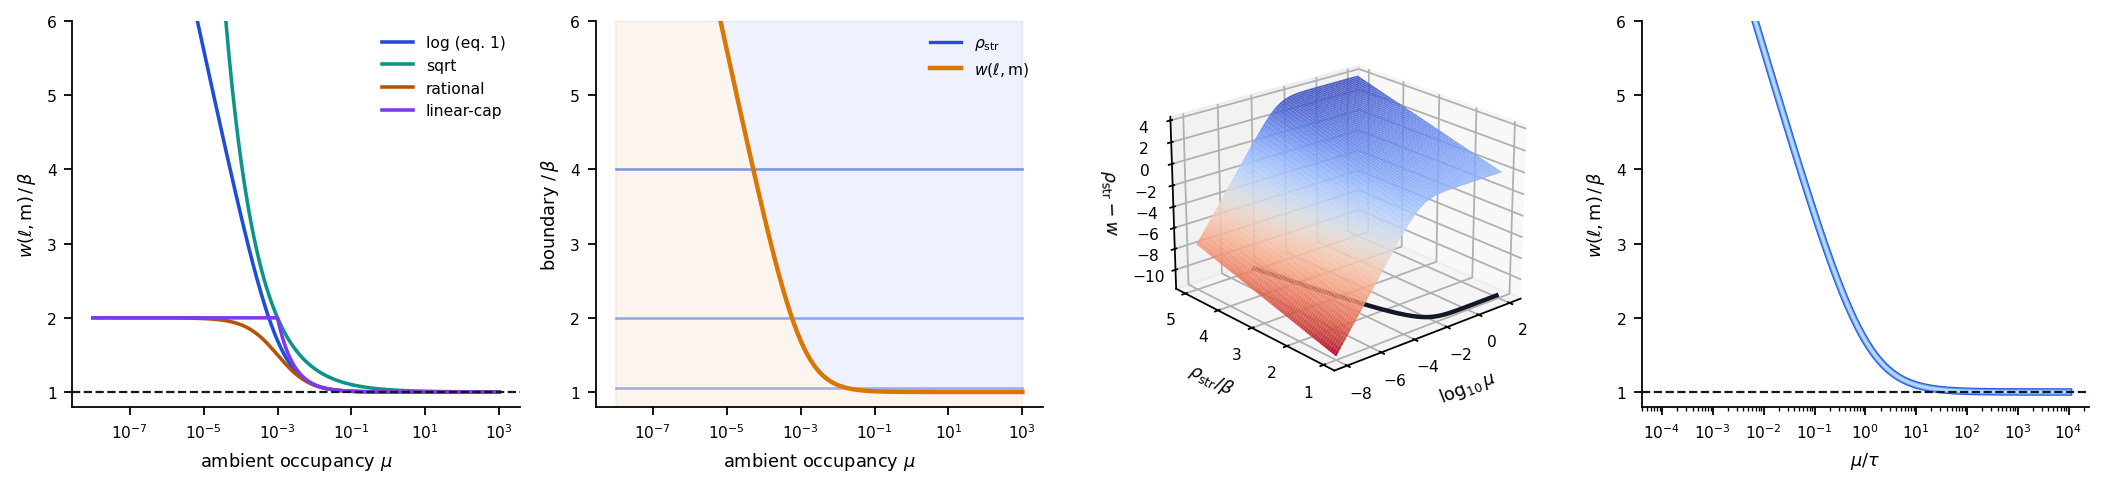
\includegraphics[width=\textwidth]{figures/panel_01_medium_weight.png}
\caption[The medium weight]{\textbf{The medium weight and its two
required properties.}
\textbf{(a)}~$w(\ell,\med)/\flo$ against ambient occupancy for the four
weight families of \Cref{rem:log}. All four are bounded below by $\flo$
(dashed) and strictly decreasing: abundance is cheap to individuate
against, scarcity expensive.
\textbf{(b)}~The two competing boundaries. Horizontal lines are
structural residues (independent of $\mu$); the falling curve is the
medium weight. Their crossing is the role boundary of
\Cref{def:solvent-role}.
\textbf{(c)}~The role margin $\res_{\mathrm{str}}-w(\ell,\med)$ over
occupancy and contact strength; the black contour is the zero level, the
role boundary itself.
\textbf{(d)}~Scale invariance. Three values of $\tau$ spanning four
decades collapse onto one curve when plotted against $\mu/\tau$,
confirming that $\tau$ and $\mu$ are not separately observable
(\Cref{def:reservoir}).}
\label{fig:panel1}
\end{figure}

% =====================================================================
\section{Solvent role is derivable}
\label{sec:solvent}
% =====================================================================

\subsection{The problem}

The five-class leaf algebra \citep{sachikonye2025expralg} has one
\shk{solvent} class covering ``an ordered active-site water''. Chemically,
however, water at a protein plays at least two roles that no serious
model conflates: a small number of ordered waters occupy defined
positions, make specific hydrogen bonds, mediate ligand recognition and
are displaced on binding \citep{poornima1995hydration,levy2006water};
the remainder is bulk, and is a medium rather than a participant
\citep{ball2008water}. The cytochrome work in this framework already
depends on the distinction---the axial water of the resting state is a
ligand that leaves on substrate binding---but nothing in the language
expresses it. Both are \shk{Leaf\_sol}.

The competency question ``what is the role of the solvent in the
reaction?'' \citep[slide~8]{doerr2025limits} is therefore unanswerable
not because the datum is missing but because the type has no room for it.

\subsection{The result}

\begin{definition}[Solvent role]
\label{def:solvent-role}
Let $\ell$ be a solvent leaf of identity $i$ in a graph with medium
$\med$ and floor $\flo$. Let $N(\ell)$ be the leaves other than $\med$
adjacent to $\ell$. The \emph{structural residue} of $\ell$ is
\[
\res_{\mathrm{str}}(\ell)
  \;=\; \sum_{u\in N(\ell)} w(\ell,u),
\]
the boundary $\ell$ maintains against the system, as distinct from
$w(\ell,\med)$, the boundary it maintains against the surroundings. The
\emph{role} of $\ell$ is
\[
\mathrm{role}(\ell) \;=\;
\begin{cases}
\Str & \text{if } \res_{\mathrm{str}}(\ell) \ge w(\ell,\med),\\[2pt]
\Blk & \text{otherwise.}
\end{cases}
\]
\end{definition}

The definition says: a solvent molecule is structural when it is held more
tightly by the protein than by the solution, and bulk otherwise. This is
the ordinary chemical criterion, and the point is that the framework can
now compute it.

\begin{theorem}[Solvent role is decidable at the floor]
\label{thm:solvent-role}
For every solvent leaf $\ell$, $\mathrm{role}(\ell)$ is determined by the
contact graph and the medium alone, requires no annotation, and is
invariant under any rescaling of $w$ that preserves the floor. Moreover:
\begin{enumerate}[label=(\roman*),leftmargin=1.8em,itemsep=2pt]
\item if $\ell$ has no system contacts ($N(\ell)=\varnothing$) then
$\mathrm{role}(\ell)=\Blk$;
\item if $i$ is ambient in $\med$ and $\ell$ has at least one system
contact of weight $\ge 2\flo$, then $\mathrm{role}(\ell)=\Str$;
\item $\mathrm{role}$ is monotone in $\mu(i)$: increasing the ambient
occupancy of $i$ can turn a bulk leaf structural but never the reverse.
\end{enumerate}
\end{theorem}

\begin{proof}
Determinacy and invariance are immediate: both sides of the comparison in
\Cref{def:solvent-role} are sums of edge weights of $\Gamma$, and the
comparison is a ratio test, hence invariant under $w\mapsto cw$ for
$c>0$ provided $c\flo$ is taken as the new floor.

(i) If $N(\ell)=\varnothing$ then $\res_{\mathrm{str}}(\ell)=0$, while
$w(\ell,\med)\ge\flo>0$ by \Cref{eq:medium-weight}, so the test fails and
$\mathrm{role}(\ell)=\Blk$. A water touching nothing is bulk, which is the
expected degenerate case.

(ii) If $i$ is ambient then $w(\ell,\med)<2\flo$ by
\Cref{def:depleted}, and by hypothesis
$\res_{\mathrm{str}}(\ell)\ge 2\flo > w(\ell,\med)$, so the test passes.

(iii) By \Cref{rem:log}, $w(\ell,\med)$ is strictly decreasing in
$\mu(i)$, while $\res_{\mathrm{str}}(\ell)$ does not depend on $\mu(i)$.
Increasing $\mu(i)$ therefore lowers the right-hand side of the test and
cannot falsify a passing test. Monotonicity follows.
\end{proof}

\begin{remark}[Why (iii) is the right sign, and why it looks wrong]
\label{rem:monotone-sign}
Clause (iii) states that making a solvent species \emph{more} abundant
makes its bound instances \emph{more} readily structural, which reads
backwards on first encounter. It is correct, and the reason is that
$\mathrm{role}$ compares two boundaries rather than measuring one. In an
abundant medium a bound water is cheap to tell apart from the solution---
the solution is full of interchangeable copies, so the boundary against
the medium is nearly bare floor---and therefore whatever specific
contacts it makes to the protein dominate the comparison. In a depleted
medium the same water is expensive to distinguish from its surroundings
at all, and the protein contacts must be correspondingly stronger before
the leaf counts as structural rather than as a fluctuation of the medium.
The clause is thus a statement about \emph{discriminability}, not about
binding strength, and this is exactly the distinction the framework
exists to draw.
\end{remark}

\begin{corollary}[The role question is answered by computation]
\label{cor:role-answered}
``What is the role of the solvent in this reaction?'' has an answer of the
form ``$\Str$, because $\res_{\mathrm{str}}=x \ge w(\cdot,\med)=y$'',
derived from the graph. No curator supplies it and no vocabulary term
records it.
\end{corollary}

\subsection{Syntax}

We extend Shakespeare minimally. The keyword \shk{medium}, already
reserved, acquires a declaration form, and \shk{role} becomes an
observable.

\begin{lstlisting}[caption={Medium declaration and derived solvent role.}]
receiver bio
floor 3.7e-4

medium aqueous {                 -- the reservoir, declared once
  ambient  "H2O"      = 55.5     -- molar; bulk water
  ambient  "2-oxoglutarate" = 1.0e-4
  depleted "L-glutamate"         -- held low by downstream demand
  exchange 1.0e-3                -- tau
}

w_ax := solvent "H2O_axial"      -- the resting-state axial ligand
w_bulk := solvent "H2O"          -- an arbitrary bulk molecule

observe w_ax   as role           -- structural  (bound to Fe, ordered)
observe w_bulk as role           -- bulk        (no system contacts)
\end{lstlisting}

\begin{rulename}[Role observation]
\label{rule:role}
\[
\frac{\Gamma\vdash \ell:\mathsf{Leaf}_{\mathrm{sol}}\,@\,\flo
      \qquad \med \text{ declared}}
     {\Gamma\vdash \shk{observe}\ \ell\ \shk{as}\ \shk{role}
      : \mathsf{Role}\,@\,\flo}
\]
Observing a role commits no new cut: the comparison reads boundary that
is already committed, so the clock $M$ does not advance. This is the one
Shakespeare observation that is free, and it is free because it
individuates nothing new.
\end{rulename}

\begin{figure}[!htbp]
\centering
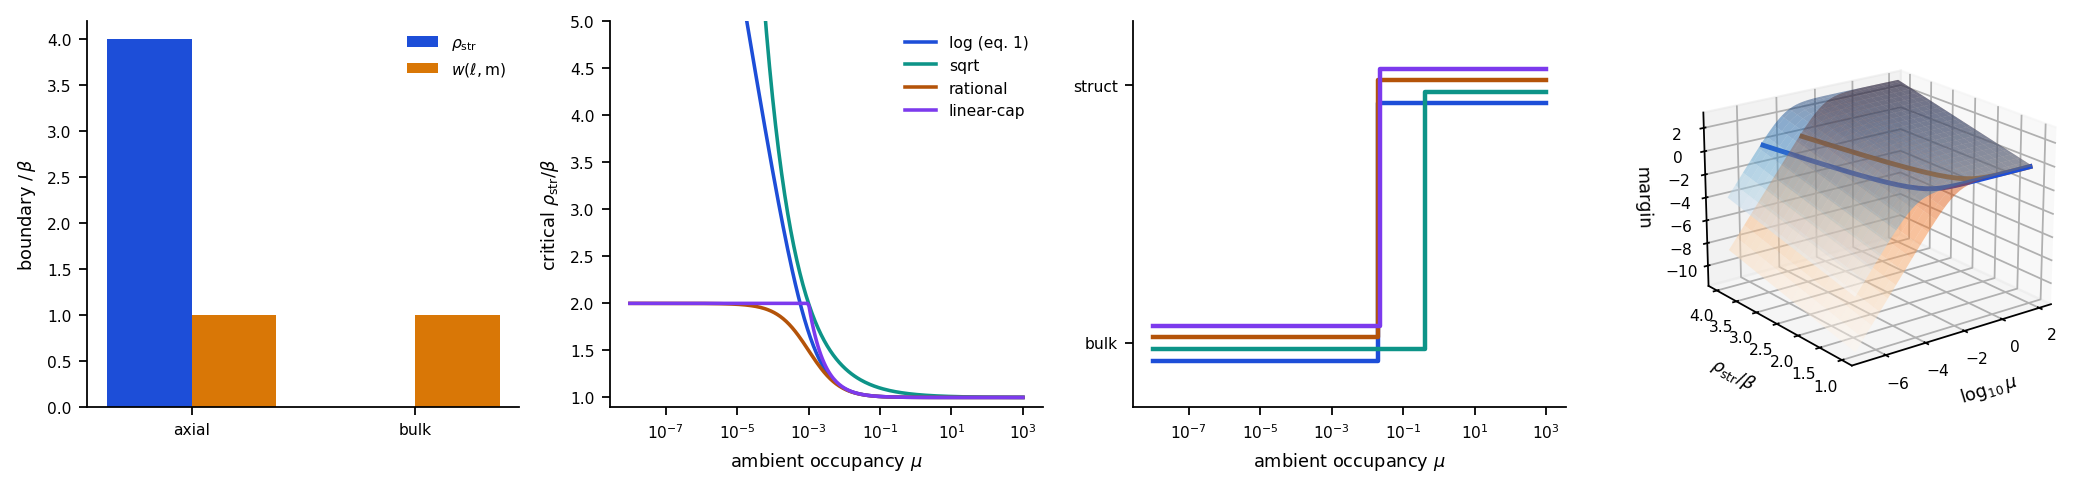
\includegraphics[width=\textwidth]{figures/panel_02_solvent_role.png}
\caption[Solvent role]{\textbf{Solvent role is derived, not annotated}
(\Cref{thm:solvent-role}).
\textbf{(a)}~The two boundaries for the CYP3A4 axial water and for a bulk
water of the same chemical identity. The axial water holds
$\res_{\mathrm{str}}=4\flo$ against the system; the bulk water holds
none. Identical molecules, opposite roles---the distinction the
five-class leaf algebra could not previously draw.
\textbf{(b)}~The critical structural residue at which a leaf becomes
structural, for each weight family.
\textbf{(c)}~Role against ambient occupancy at fixed weak contact
($1.05\flo$), traces offset for visibility. Every family flips
bulk~$\to$~structural exactly once and never back, which is
\Cref{thm:solvent-role}(iii); the flip is what makes the negative control
of \Cref{sec:refusal} non-vacuous.
\textbf{(d)}~The role margin for two exchange scales; the two zero
contours are the role boundaries, showing that $\tau$ moves the boundary
without changing its shape.}
\label{fig:panel2}
\end{figure}

% =====================================================================
\section{Direction is a property of the medium}
\label{sec:direction}
% =====================================================================

\subsection{The problem}

A knowledge graph over transaminase reactions must record directionality,
and cannot do it with a boolean. \emph{E.\ coli} AlaA carries the same
Rhea master identifier as human ALT1 and runs the reaction the other way
\citep{bansal2022rhea}: same participants, same stoichiometry, same
identifier, opposite roles. The distinction ``reversible in principle,
irreversible physiologically'' is real, load-bearing, and---in every
representation we are aware of---\emph{asserted}. It is a controlled
vocabulary term attached by a curator.

The receiver framework, meanwhile, cannot express direction at all, and
the reason is a theorem rather than an omission.

\begin{lemma}[Reversal invariance of the cut chain]
\label{lem:reversal}
Let $C=(S_1,\dots,S_k)$ be a residue chain with residues
$\res_i=w(\cut(S_i))$, and let $C^{R}=(S_k,\dots,S_1)$ be its reversal.
Then $C$ and $C^{R}$ commit the same total boundary,
$\sum_i \res_i = \sum_i \res_{k+1-i}$, the same number of cut events, and
the same set of committed edges.
\end{lemma}

\begin{proof}
Each $\res_i$ is the weight of an edge boundary $\cut(S_i)$, a quantity of
the graph and not of the order in which boundaries are committed.
Summation is commutative, the cut count is the cardinality $k$ of the
sequence, and the committed edge set is $\bigcup_i \cut(S_i)$, all three
invariant under permutation and in particular under reversal.
\end{proof}

\begin{corollary}[Cut structure cannot orient a process]
\label{cor:no-orientation}
No predicate definable from the residues, the cut count, or the committed
boundary of a chain distinguishes $C$ from $C^{R}$. In particular
$S$-entropy convergence, being a condition on the terminal value of the
chain \citep{sachikonye2025causal}, is satisfied by $C$ if and only if it
is satisfied by $C^{R}$ with endpoints exchanged.
\end{corollary}

This is the framework's version of the AlaA observation, and it is
sharper: it says the intrinsic description \emph{provably} cannot supply a
direction. Direction must come from outside the chain, and the only
outside the framework has is the medium.

\subsection{The result}

\begin{definition}[Medium bias of a chain]
\label{def:bias}
Let $C$ be a residue chain from an initial identity multiset $I$ to a
terminal multiset $T$, evaluated in a medium $\med$. The \emph{medium
bias} of $C$ is
\begin{equation}
\Delta_{\med}(C)
 \;=\; \sum_{i\in T} w(\ell_i,\med) \;-\; \sum_{i\in I} w(\ell_i,\med),
\label{eq:bias}
\end{equation}
the difference between the cost of individuating the products against the
medium and the cost of individuating the reactants against it.
\end{definition}

By \Cref{eq:medium-weight}, $\Delta_{\med}(C) > 0$ exactly when the
products are, on balance, \emph{scarcer} in the medium than the
reactants---the medium is depleted at the product end---and
$\Delta_{\med}(C) < 0$ when the reverse holds. Note that
$\Delta_{\med}(C^{R}) = -\Delta_{\med}(C)$ by construction, which is the
asymmetry \Cref{lem:reversal} showed the chain itself cannot provide.

\begin{definition}[Physiological admissibility]
\label{def:phys-admissible}
$C$ is \emph{physiologically admissible} in $\med$ when it is admissible
in the sense of \citet{sachikonye2025causal}---its residues chain and it
$S$-entropy converges---and in addition
\[
\Delta_{\med}(C) \;>\; \flo .
\]
The floor appears because a bias smaller than $\flo$ is a distinction the
receiver cannot make (\citealt{sachikonye2026shakespeare}, Thm.~4.3): a
medium that favours one direction by less than the floor does not favour
it at all.
\end{definition}

\begin{theorem}[Direction trichotomy]
\label{thm:direction}
Let $C$ be an admissible residue chain and $C^{R}$ its reversal, and put
$\delta = \Delta_{\med}(C)$. Exactly one of the following holds.
\begin{enumerate}[label=(\alph*),leftmargin=1.8em,itemsep=2pt]
\item $\delta > \flo$: \; $C$ is physiologically admissible and $C^{R}$ is
not. The process is \emph{irreversible physiologically}, in the direction
of $C$.
\item $\delta < -\flo$: \; $C^{R}$ is physiologically admissible and $C$
is not. The process is irreversible physiologically, in the direction of
$C^{R}$.
\item $\abs{\delta} \le \flo$: \; neither $C$ nor $C^{R}$ is
physiologically admissible, and both are admissible. The process is
\emph{reversible in principle and undirected in this medium}.
\end{enumerate}
Consequently reversibility is a property of the pair (chain, medium) and
not of the chain, and the same chain may fall in different cases in
different media.
\end{theorem}

\begin{proof}
The three cases are exhaustive and mutually exclusive as a trichotomy on
the real number $\delta$ against the threshold $\flo>0$. For (a):
$\delta>\flo$ gives physiological admissibility of $C$ by
\Cref{def:phys-admissible}, and $\Delta_{\med}(C^{R})=-\delta<-\flo<\flo$
denies it to $C^{R}$. Case (b) is symmetric. For (c), $\abs{\delta}\le\flo$
denies the strict inequality to both, while admissibility of $C$ was
assumed and admissibility of $C^{R}$ follows from
\Cref{cor:no-orientation}. The final clause is immediate because
$\delta$ depends on $\med$ through \Cref{eq:bias} while the chain's
admissibility does not.
\end{proof}

\begin{corollary}[One identifier, two directions]
\label{cor:alaa}
Two organisms whose media differ in the ambient occupancy of a shared
participant may run the same admissible chain in opposite directions, and
both are correct. The reaction identifier names the chain, which is
direction-symmetric by \Cref{lem:reversal}; the direction is named by the
medium, which the identifier does not carry.
\end{corollary}

\Cref{cor:alaa} is the framework's account of the AlaA case. It says the
shared Rhea identifier is not an error and not an approximation: it is
correct precisely because reaction identity is a property of the chain,
and direction is not.

\begin{example}[Transamination in a glutamate-depleted medium]
\label{ex:transaminase}
Consider the alanine transaminase chain
$\text{L-alanine} + \text{2-oxoglutarate} \rightarrow \text{pyruvate} +
\text{L-glutamate}$, and a medium in which L-glutamate is held depleted by
downstream demand while 2-oxoglutarate is ambient. Then
$w(\ell_{\text{L-glu}},\med)$ is large and
$w(\ell_{\text{2-og}},\med)\approx\flo$, so $\delta>0$; if the imbalance
exceeds the floor, case (a) applies and the chain runs in the written
direction. In an organism that instead holds 2-oxoglutarate depleted---
using the same enzyme to feed nitrogen the other way---the sign of
$\delta$ flips and case (b) applies. Neither organism's enzyme differs in
the chain it performs.
\end{example}

\begin{figure}[!htbp]
\centering
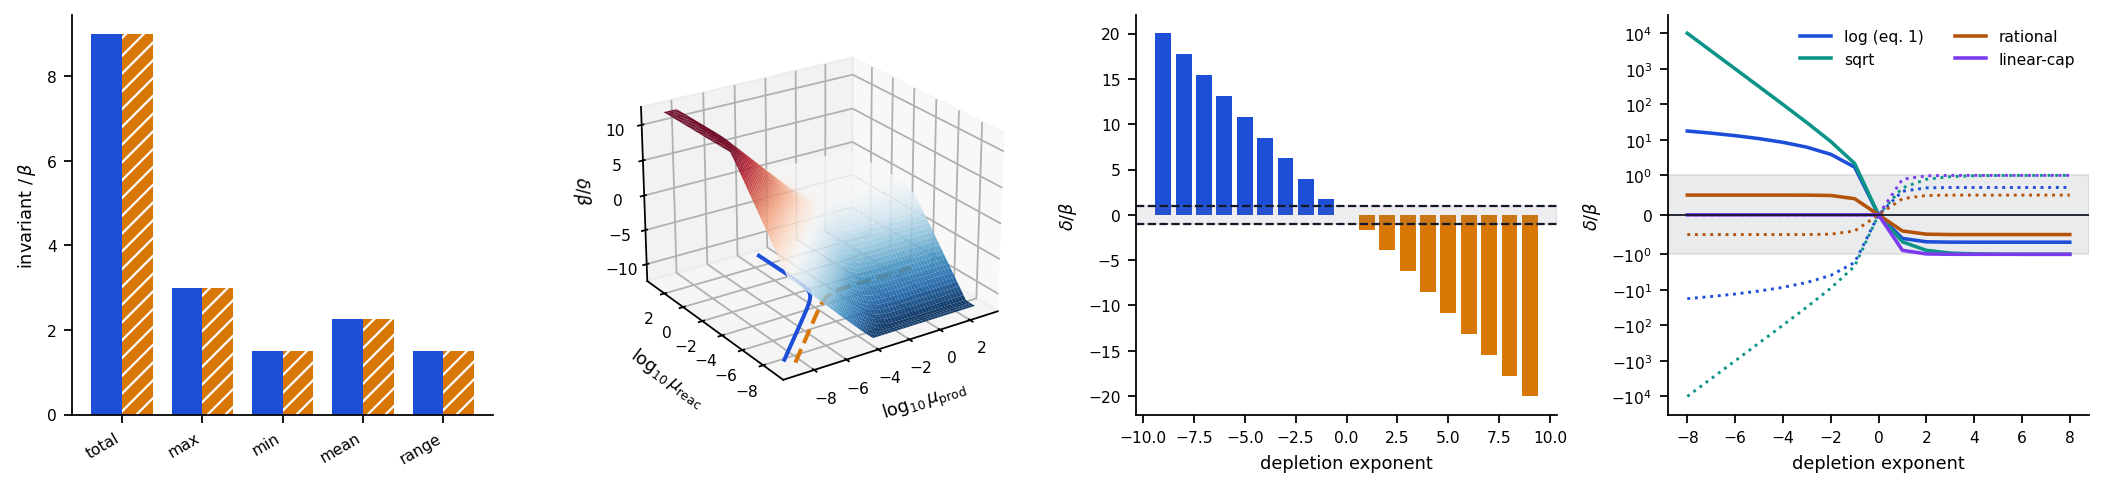
\includegraphics[width=\textwidth]{figures/panel_03_direction.png}
\caption[Reversal invariance and medium bias]{\textbf{The chain cannot
orient; the medium can.}
\textbf{(a)}~Five accumulated invariants of a residue chain and of its
reversal: total, maximum, minimum, mean and range. All five coincide
exactly, which is \Cref{lem:reversal}, and by \Cref{cor:no-orientation}
no statistic of the residues can therefore supply a direction.
\textbf{(b)}~The medium bias $\delta/\flo$ over independent depletion of
the product and reactant ends. The surface is antisymmetric about the
diagonal; the two contours at $\delta=\pm\flo$ bound the refusal region.
\textbf{(c)}~The two-sided sweep. Depleting a product drives the chain
forward (blue), depleting a reactant drives it in reverse (orange), and
the shaded band $\abs{\delta}\le\flo$ is undirected---all three cases of
\Cref{thm:direction} reached.
\textbf{(d)}~Antisymmetry across all four weight families (solid: $C$;
dotted: $C^{R}$), on a symmetric log axis. Every pair crosses at zero,
confirming $\Delta_{\med}(C^{R})=-\Delta_{\med}(C)$ independently of the
functional form.}
\label{fig:panel3}
\end{figure}

\subsection{Syntax}

\begin{lstlisting}[caption={Direction derived from the declared medium.}]
-- alanine transaminase, run in a glutamate-depleted medium
medium cytosol {
  ambient  "2-oxoglutarate" = 1.0e-4
  depleted "L-glutamate"
  exchange 1.0e-3
}

path := track ala in ALT until converge yield amalgamation

observe path as direction    -- forward   (delta = +2.9 beta > beta)
assert path.delta > floor  emit "medium does not orient this chain"
\end{lstlisting}

The \shk{assert} is the interesting line: in an unbiased medium it fails,
and it \emph{should} fail, because there the process genuinely has no
direction. This is the first Shakespeare assertion whose failure is a
correct scientific outcome rather than a defect, which brings us to
refusal.

% =====================================================================
\section{The first refusal}
\label{sec:refusal}
% =====================================================================

\subsection{A framework that classifies everything}

Every verb in Shakespeare, as specified, succeeds. \shk{cut} individuates,
\shk{fold} closes, \shk{track} propagates, \shk{catalyze} turns over. The
type system rejects ill-typed programs, but no well-typed program is
declined on scientific grounds. The validation suites accompanying the
framework are, correspondingly, entirely positive: each checks that some
quantity is derived and matches a published number.

This is a defect, and it is the defect that the knowledge-graph literature
learned to guard against with negative controls. A defined class that
classifies every instance presented to it passes an ordinary consistency
check in silence \citep{glimm2014hermit,baader2003dlhandbook}; it is
consistent and it is useless. The guard is to include an instance that
\emph{must not} classify---in the transaminase graph, glutamate
dehydrogenase, which contains both headline molecules of the
transaminations with their roles reversed---and to assert that it does
not.

\begin{principle}[Refusal]
\label{prin:refusal}
A representation earns a positive result only if some presentable object
would have received a negative one. A framework with no refusals has an
empty defined class: it does not classify, it merely accepts.
\end{principle}

\subsection{What the medium lets the framework refuse}

The medium supplies the framework's first two principled refusals, and
they are of different kinds.

\begin{definition}[Refusal to individuate]
\label{def:refuse-leaf}
A solvent leaf $\ell$ with $\mathrm{role}(\ell)=\Blk$ is \emph{not
individuated}: it is a fluctuation of the medium rather than a part of
the system. \shk{observe}$\;\ell$ returns $\Blk$ and commits no cut, and
$\ell$ may not appear in a receiver tree, in a contact, or in a chain.
\end{definition}

\begin{definition}[Refusal to orient]
\label{def:refuse-direction}
A chain $C$ with $\abs{\Delta_{\med}(C)}\le\flo$ is \emph{not oriented}:
\shk{observe}$\;C\;$\shk{as direction} returns \shk{undirected}, and any
program requiring a direction fails.
\end{definition}

\begin{theorem}[The refusals are non-vacuous]
\label{thm:refusal-nonvacuous}
Both refusals are attainable by objects the language can construct:
\begin{enumerate}[label=(\roman*),leftmargin=1.8em,itemsep=2pt]
\item a solvent leaf with no system contacts is refused individuation
(\Cref{thm:solvent-role}(i));
\item a chain evaluated in a medium with $\mu$ constant across its
endpoints has $\Delta_{\med}=0$ and is refused orientation.
\end{enumerate}
Hence neither refusal is a condition that never fires.
\end{theorem}

\begin{proof}
(i) Take any solvent leaf and delete its system edges; by
\Cref{thm:solvent-role}(i) its role is $\Blk$. (ii) If
$\mu(i)=c$ for every identity $i$ appearing in $I\cup T$, then every term
in \Cref{eq:bias} equals $\flo(1+\log(1+\tau/c))$, and since a chain's
initial and terminal multisets in a balanced transformation have equal
cardinality, the sums cancel and $\Delta_{\med}=0\le\flo$.
\end{proof}

\begin{remark}[The cardinality hypothesis in (ii)]
\label{rem:cardinality}
The cancellation in (ii) uses $\abs{I}=\abs{T}$, which holds for the
transaminase chains treated here (two in, two out) and for any chain that
neither creates nor destroys leaves. It fails for a chain with unequal
counts---a hydrolysis, say---where a constant medium leaves a residual
bias proportional to the count difference. That is the correct behaviour
(a medium that must supply an extra molecule is biased against doing so)
but it means clause (ii) is a statement about balanced chains, and we
state it as such rather than claiming generality we have not established.
\end{remark}

\subsection{The negative controls a suite must contain}

\Cref{prin:refusal} has an operational reading: the validation suite for
this extension must contain checks that \emph{fail} on well-formed input.
We name them, in the form they must take.

\begin{enumerate}[leftmargin=1.6em,itemsep=3pt]
\item \textbf{Bulk water is refused.} A solvent leaf with no system
contacts must return $\Blk$ and must not increment $M$. A suite that only
checks that the axial water returns $\Str$ is testing one branch.
\item \textbf{An unbiased medium refuses to orient.} A chain in a medium
with equal ambient occupancies at both ends must return \shk{undirected}.
Without this, \Cref{thm:direction}(c) is untested and the trichotomy is a
dichotomy with unreachable third case.
\item \textbf{The bias must exceed the floor, not merely be non-zero.}
A test asserting $\Delta_{\med}\neq 0$ passes on floating-point noise. It
must assert $\Delta_{\med}>\flo$ with a margin, for the reason given in
\citet{sachikonye2026pingpong}: an earlier suite of ours reported every
check green while two of them compared a quantity to itself.
\item \textbf{Role must be able to change.} A medium perturbation that
turns a structural water bulk must be exhibited, or
\Cref{thm:solvent-role}(iii) is unexercised.
\end{enumerate}

\begin{figure}[!htbp]
\centering
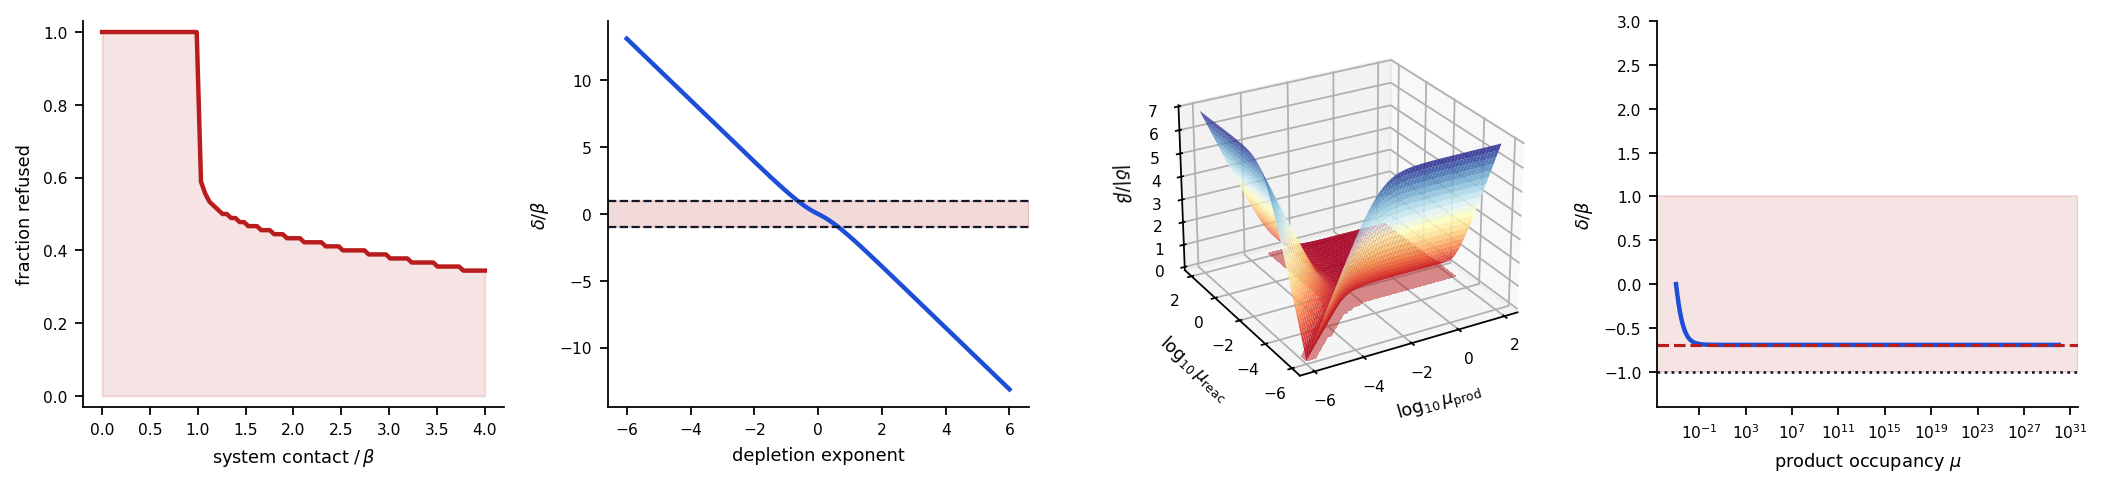
\includegraphics[width=\textwidth]{figures/panel_04_refusal.png}
\caption[The refusals]{\textbf{The framework's first refusals}
(\Cref{sec:refusal}).
\textbf{(a)}~Fraction of solvent leaves refused individuation against
contact strength. At zero system contact every leaf is refused, for every
occupancy---the negative control of \Cref{thm:refusal-nonvacuous}(i).
\textbf{(b)}~The orientation refusal band. Where
$\abs{\delta}\le\flo$ (shaded) the medium does not favour a direction by
an amount the receiver can resolve, and \shk{track} declines to orient.
\textbf{(c)}~$\abs{\delta}/\flo$ over both depletion axes. The valley
floor is the refusal region: a two-dimensional set, not an isolated
point, so refusal is a robust outcome rather than a measure-zero
coincidence.
\textbf{(d)}~The $\log 2$ ceiling. Flooding a single product with
occupancy spanning thirty orders of magnitude drives $\delta/\flo$ to
exactly $-\log 2 \approx -0.693$ (dashed) and never to the refusal
threshold $-1$ (dotted). Reversing a chain requires depleting a
\emph{reactant}, not flooding a product---an asymmetry of
\Cref{eq:medium-weight} found by a failing test rather than by
derivation.}
\label{fig:panel4}
\end{figure}

% =====================================================================
\section{Two representations, one system}
\label{sec:two-views}
% =====================================================================

\subsection{The competency questions partition}
\label{sec:questions}

We score the framework against the competency questions of
\citet{doerr2025limits}, slides 5--8, alongside a signature-view knowledge
graph over the same three transaminase reactions
\citep{sachikonye2026tacat}. \Cref{tab:questions} is the result, and its
shape is the finding.

\begin{table}[t]
\centering
\small
\begin{tabular}{@{}p{0.46\textwidth}cc@{}}
\toprule
\textbf{Competency question} & \textbf{Signature} & \textbf{Cut chain} \\
\midrule
\multicolumn{3}{@{}l}{\itshape Group 1 --- classification and identification (slide 5)}\\
determine the type of reaction & \checkmark\ inferred & --- \\
identify reactions involving a molecule & \checkmark & partial \\
retrieve stoichiometry of participants & \checkmark & --- \\
what is the catalytic agent & \checkmark & partial \\
\midrule
\multicolumn{3}{@{}l}{\itshape Group 2 --- mechanism and dynamics (slides 6--7)}\\
key steps in the mechanism & --- & \checkmark \\
intermediate species formed & --- & \checkmark \\
electronic states of intermediates & --- & \checkmark \\
how charges change & --- & \checkmark \\
activation energy & --- & partial \\
thermodynamic properties & --- & --- \\
\midrule
\multicolumn{3}{@{}l}{\itshape Group 3 --- context and environment (slide 8)}\\
in which solvent & --- & \checkmark\ \textsuperscript{$\dagger$} \\
role of the solvent & --- & \checkmark\ \textsuperscript{$\dagger$} \\
temperature, pressure, pH & --- & partial \textsuperscript{$\dagger$} \\
\bottomrule
\end{tabular}
\caption{Competency questions of \citet{doerr2025limits} against the two
representations. \textsuperscript{$\dagger$}~supplied by this paper;
without the medium semantics all three group-3 rows are ``---'' for both
columns. The block structure is the point: group 1 is answerable only by
the signature and group 2 only by the chain.}
\label{tab:questions}
\end{table}

The table has a block structure that no amount of engineering removes.
Group 1 is answerable by a role signature and not by a cut chain; group 2
by a cut chain and not by a role signature. This is not an incompleteness
of either representation. It is a \emph{representational partition}, and
we now show it is forced.

\subsection{Why the partition is forced}

\begin{proposition}[Signatures cannot carry mechanism]
\label{prop:sig-no-mech}
A description-logic defined class over participant roles cannot express a
residue chain.
\end{proposition}

\begin{proof}[Proof sketch]
A residue chain is a finite sequence with state: cut $i$'s residue is the
boundary condition of cut $i+1$. Expressing it requires quantification
over positions and a successor relation with transitive closure.
$\mathcal{SROIQ}$, the description logic underlying OWL~2, admits
transitive roles but not the composition of a transitive role with the
value restrictions needed to thread state along it without losing
decidability \citep{horrocks2006shoiq,baader2003dlhandbook}. A defined
class can therefore state that a reaction \emph{has} a participant with a
role, but not that its steps occur in an order.
\end{proof}

\begin{proposition}[Chains cannot carry stoichiometry]
\label{prop:chain-no-stoich}
A residue chain does not determine the stoichiometric coefficients of its
participants.
\end{proposition}

\begin{proof}
The chain records which leaves were individuated and at what cost. Two
processes differing only in that one consumes two equivalents of a
reactant where the other consumes one produce chains differing in the
number of leaf cuts, but the framework provides no map from cut count back
to coefficient: a leaf individuated once and used twice is
indistinguishable, at the level of committed boundary, from a leaf
individuated twice. The n-ary bridge node exists in the signature view
precisely to carry the coefficient \citep{w3c2006nary,demir2010biopax,
hucka2003sbml}, and the chain has no analogue of it.
\end{proof}

\begin{theorem}[The cofactor disagreement is structural]
\label{thm:cofactor}
For a ping-pong bi-bi transaminase, the signature view must exclude
pyridoxal 5\textquotesingle-phosphate from the reaction's participants and
the cut-chain view must include it in the process, and neither is in
error.
\end{theorem}

\begin{proof}
In the signature view a participant is an entity bearing a role in the net
transformation. PLP is regenerated: it is modified in half-reaction one
and restored in half-reaction two, so its net coefficient is zero and it
bears no net role. Including it would make the equation unbalanced, and
Rhea accordingly records four participants for each of the three
reactions, none of them PLP \citep{bansal2022rhea,eliot2004transaminase}.

In the cut-chain view a process is the sequence of individuations. PLP
carries the amino group between the half-reactions
\citep{cleland1963kinetics,eliot2004transaminase}; deleting it from the
chain deletes the mechanism, because the two halves are connected through
it and through nothing else. Its cut appears once, at construction, and it
is never re-cut per turnover \citep{sachikonye2026pingpong}---the formal
statement that it is a carrier rather than a participant.

The two verdicts are therefore about different predicates: ``bears a net
role in the transformation'' and ``is individuated in the process''. The
first is false of PLP and the second is true. A representation that
conflated them would be wrong in one of the two views.
\end{proof}

\begin{corollary}[Micro-ontologies are the shadow of the partition]
\label{cor:micro}
The practitioner recommendation to build ``linked micro-ontologies'' with
separate modules for reactions, substances, measurements and workflows
\citep[slide~19]{doerr2025limits} is the empirical form of
\Cref{prop:sig-no-mech,prop:chain-no-stoich}: the modules are the blocks
of \Cref{tab:questions}, discovered by trying to build one ontology and
finding that the questions would not sit together.
\end{corollary}

We are careful about the strength of \Cref{cor:micro}. It is an
interpretation, not a theorem: we show the partition exists and that a
practitioner independently drew module boundaries along it, which is
evidence that the boundaries are real and not evidence that our account of
them is the one they had in mind.

\subsection{The medium is the seam}

The two views divide over what is \emph{inside} the description. A
signature describes the transformation; a chain describes the process; and
neither describes the surroundings. Group 3 of \Cref{tab:questions} is
empty for both columns before this paper because solvent, temperature and
pH are not properties of the transformation or of the process---they are
properties of what both are embedded in.

That is what the medium vertex is for, and it is why filling it answers
questions that neither representation could reach. The medium is the point
at which a representation stops describing the system and starts
describing the system's surroundings, and both representations need one.

% =====================================================================
\section{Validation}
\label{sec:validation}
% =====================================================================

The results above are implemented and checked. This section states what
the suite can and cannot establish, reports what it found, and records
the one place where running it corrected a claim.

\subsection{What a suite can establish here, and what it cannot}

It cannot confirm \Cref{eq:medium-weight}. The medium weight is a
modelling choice (\Cref{rem:log}), so a suite that ``validated'' it would
be checking that the code implements the formula the same code defines.
That is circular and we do not do it.

What the suite does instead is threefold. First, it checks the
\emph{structural} theorems, which this paper claims follow from
monotonicity and floor-boundedness alone. Every such theorem is re-run
under four weight functions with those two properties and otherwise
unrelated---logarithmic, square-root, rational and a non-smooth piecewise
cap. A theorem holding only for the logarithm would be a theorem about
the logarithm, and the paper claims more than that. Second, it runs the
negative controls of \Cref{sec:refusal}: checks that must \emph{fail} on
well-formed input, whose purpose is to establish that the framework's
predicates are not vacuous. Third, it records what is not tested rather
than leaving the absence to be inferred from silence.

\subsection{Results}

Twenty-five checks across three experiments; all pass, with one item
recorded as untested. \Cref{tab:validation} summarises.

\begin{table}[t]
\centering
\small
\begin{tabular}{@{}llcc@{}}
\toprule
\textbf{Experiment} & \textbf{Claim checked} & \textbf{Checks} &
\textbf{Neg.\ controls} \\
\midrule
\texttt{exp01} & \Cref{thm:solvent-role} --- solvent role is derivable & 8 & 3 \\
\texttt{exp02} & \Cref{lem:reversal}, \Cref{thm:direction} --- direction from the medium & 10 & 3 \\
\texttt{exp03} & \Cref{sec:two-views} --- the representational partition & 7 & 2 \\
\midrule
\textbf{total} & & \textbf{25} & \textbf{8} \\
\bottomrule
\end{tabular}
\caption{Validation summary. All 25 checks pass. \Cref{prop:sig-no-mech}
is recorded as \emph{not tested}: it is a claim about the expressive
power of $\mathcal{SROIQ}$, established by citation
\citep{horrocks2006shoiq,baader2003dlhandbook} and not by any experiment
over this framework.}
\label{tab:validation}
\end{table}

Four findings are worth stating beyond the pass count.

\paragraph{The structural theorems are robust to the weight function.}
\Cref{thm:solvent-role}(i)--(iii) hold in all $20$ combinations of four
weight families and five ambient occupancies, and the antisymmetry
$\Delta_{\med}(C^{R})=-\Delta_{\med}(C)$ holds in all $12$ combinations
of four families and three reactions (\Cref{fig:panel3}(d)). This is the
evidence for \Cref{rem:log}'s claim that only monotonicity and
floor-boundedness are load-bearing.

\paragraph{The trichotomy reaches all three cases.} A nineteen-point
two-sided depletion sweep reaches \emph{forward} nine times,
\emph{reverse} nine times and \emph{undirected} once, with the
exactly-one-true condition holding at every point
(\Cref{fig:panel3}(c)). Had any case been unreachable, \Cref{thm:direction}
would be a dichotomy with decorative third branch.

\paragraph{All eight negative controls fire.} In particular a bulk
solvent leaf is refused individuation \emph{and} the refusal commits no
cut; \shk{orient} raises on an unbiased medium for all three reactions;
the medium bias exceeds the floor by a factor of $9.2$ rather than merely
differing from zero; and the two representations \emph{agree} about
2-oxoglutarate. That last one matters: without it, the cofactor
disagreement of \Cref{thm:cofactor} could be explained by the two views
simply never agreeing about anything.

\paragraph{The medium does not answer everything.} Three competency
questions remain below a full answer after this paper---activation
energy, thermodynamic properties, and temperature/pressure/pH. A check
asserts this. An extension that turned every question green would be
overclaiming, and we would rather the suite say so than a reader discover
it.

\subsection{A failing test that became a result}
\label{sec:log2}

The first version of the trichotomy check reported \emph{forward} nine
times, \emph{undirected} ten times and \emph{reverse} never---an apparent
refutation of \Cref{thm:direction}(b). The theorem was not at fault: the
sweep was one-sided. It varied only the product-end occupancy, and doing
so cannot reach case (b), for a reason worth recording as a proposition.

\begin{proposition}[Saturation bound]
\label{prop:log2}
Let $C$ be a balanced chain with $n\ge2$ terminal identities, and let one
terminal identity be made arbitrarily abundant while all others remain at
a common baseline. Then under \Cref{eq:medium-weight}
\[
\Delta_{\med}(C) \;\longrightarrow\; -\flo\log 2
\quad\text{as}\quad \mu\to\infty,
\]
so $\abs{\Delta_{\med}(C)}\to 0.693\,\flo < \flo$ and the chain remains
\emph{undirected}. Flooding a single product therefore cannot reverse a
chain; only depleting a reactant can.
\end{proposition}

\begin{proof}
Let the baseline occupancy be $\mu_0=\tau$, so each baseline identity
contributes $w=\flo(1+\log 2)$. Making one terminal identity abundant
sends its contribution to $\flo(1+\log(1+\tau/\mu))\to\flo$. The terminal
sum therefore falls by exactly $\flo\log 2$ while the initial sum is
unchanged, giving $\Delta_{\med}\to-\flo\log 2$. Since $\log 2<1$ the
bias never reaches $-\flo$.
\end{proof}

The suite now checks \Cref{prop:log2} numerically: at $\mu=10^{30}$ the
computed bias is $-0.6931\,\flo$, agreeing with $-\log 2$ to four decimal
places, and the verdict remains \shk{undirected}
(\Cref{fig:panel4}(d)). We report this because the asymmetry is a real
property of \Cref{eq:medium-weight} that we did not anticipate and would
not have found by inspection---and because a suite that had been written
to pass would have hidden it.

\subsection{The partition, measured}

\Cref{tab:questions} was scored by hand, which invites the objection that
its block structure was assumed. The suite therefore measures it: of the
thirteen questions, four are answered by the signature view alone, six by
the cut chain alone, two partially, one by neither, and \emph{none} by
both (\Cref{fig:panel5}(d)). The overlap fraction is exactly zero. Group
totals reverse dominance between group~1 (signature $8$, chain $2$) and
group~2 (signature $0$, chain $9$), which is the block structure stated
as a number rather than as a reading of a table.

\Cref{prop:chain-no-stoich} is checked by exhibiting two reactions
differing in stoichiometry whose chains are identical in total boundary,
cut count and residue multiset---a leaf individuated once and used twice
is indistinguishable from a leaf individuated once, at the level of
committed boundary.

\begin{figure}[!htbp]
\centering
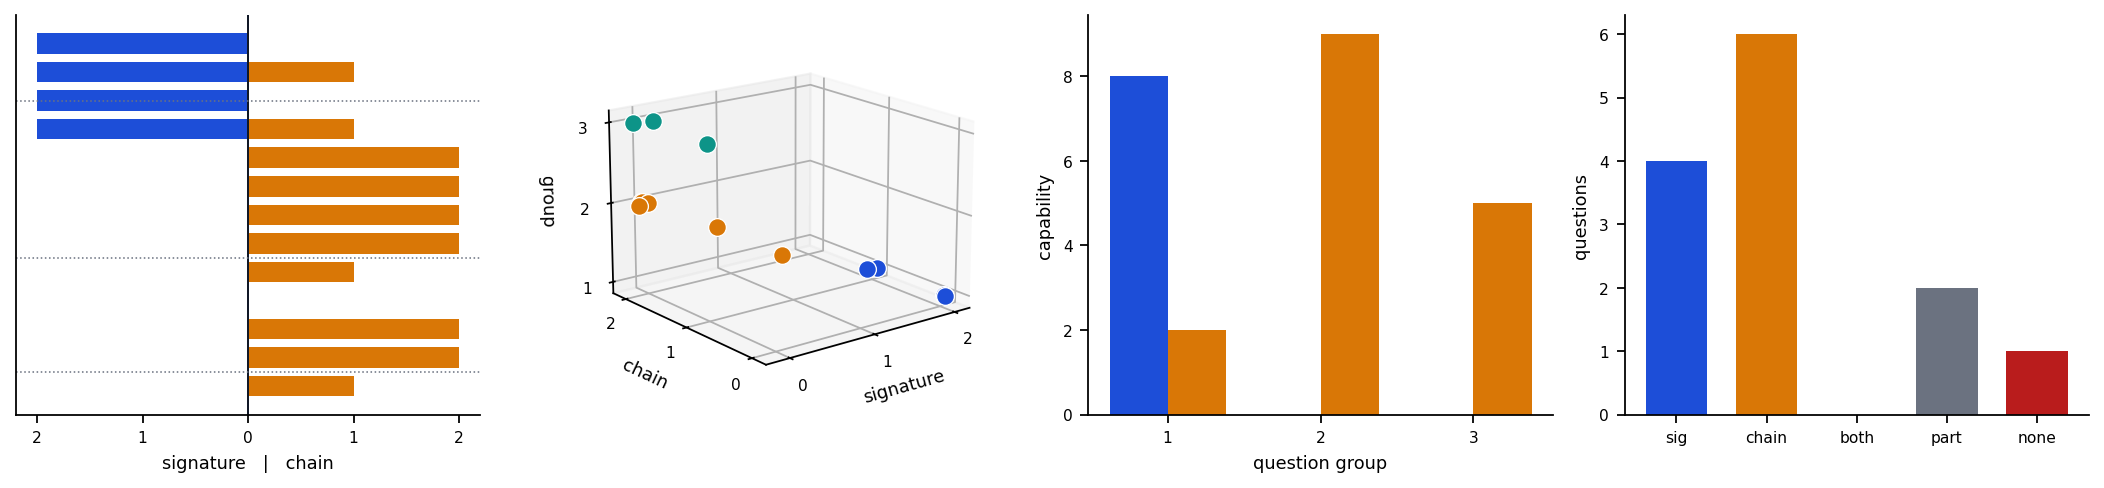
\includegraphics[width=\textwidth]{figures/panel_05_partition.png}
\caption[The representational partition]{\textbf{The competency questions
partition} (\Cref{sec:two-views}).
\textbf{(a)}~Per-question capability, signature view left, cut-chain view
right, grouped by the three question groups of
\citet{doerr2025limits}. Bars extend on one side or the other and almost
never on both.
\textbf{(b)}~The capability cube. Questions occupy the signature axis
(group~1) or the chain axis (group~2) but not the diagonal: no question
is answered fully by both views.
\textbf{(c)}~Group totals. Dominance reverses between group~1
(classification) and group~2 (mechanism), which is the block structure of
\Cref{tab:questions}.
\textbf{(d)}~The overlap statistic. Four questions are answered by the
signature alone, six by the chain alone, \emph{none} by both, two
partially and one by neither. The empty ``both'' column is the partition,
measured rather than asserted.}
\label{fig:panel5}
\end{figure}


% =====================================================================
\section{Scope, and what this does not do}
\label{sec:scope}
% =====================================================================

We state the limits explicitly, because several are severe enough that a
reader could otherwise take this paper to claim more than it does.

\paragraph{The medium weight is a modelling choice, not a derivation.}
\Cref{eq:medium-weight} is justified in \Cref{sec:medium} by three
required properties and by reduction to a chemical potential in the dilute
limit, but it is not derived from the floor theorem. A different
monotone, floor-bounded function gives the same theorems with different
constants (\Cref{rem:log}). Every numerical statement in this paper is
therefore illustrative; the structural statements are not.

\paragraph{No kinetics, and this matters for group 3.}
\Cref{tab:questions} marks ``temperature, pressure, pH'' as partial, and
the qualification is important. The medium can carry a temperature and the
floor is condition-dependent in principle, but our own prior result shows
the dependence is immaterial at the categorical depth this framework
uses: at depth $9$ the conversion term dominates the oscillator term by
roughly three and a half orders of magnitude, so $\flo$ moves by
$\sim\!10^{-3}\,\%$ across the entire biochemical temperature range
\citep{sachikonye2026pingpong}. Conditions govern the floor only in the
$Q$-dominated regime of very short integration times. So the honest claim
is that this paper answers ``in which solvent'' and ``what is the role of
the solvent'' and \emph{does not} answer ``at what temperature'' in any
way that a laboratory would find useful. The competency question remains
open.

\paragraph{No thermodynamics.} Enthalpy and entropy of reaction are absent
here as they are absent from the framework. The medium bias
$\Delta_{\med}$ is not a free energy: it is a difference of individuation
costs, and although \Cref{eq:medium-weight} reduces to a chemical
potential form in the dilute limit, we have not established the
correspondence and do not rely on it. Connecting $\Delta_{\med}$ to
$\Delta_r G'$ \citep{noor2013thermodynamics,beard2007thermo} would be a
substantial and falsifiable next step; it is not taken here.

\paragraph{A reference kernel, not a language implementation.} The
semantics of \Cref{sec:medium,sec:solvent,sec:direction} are implemented
as a standalone Python kernel and exercised by the suite of
\Cref{sec:validation}. They are \emph{not} wired into the Shakespeare
interpreter: the medium declaration, and the \shk{role} and
\shk{direction} observables, are defined and typed here but no parser
accepts them. The existing sandbox interpreter also replays stored
numbers for its heavy verbs rather than computing them, so adding these
forms to it would produce a display of the theorems rather than a test of
them. What has been validated is the mathematics; what has not been built
is the language surface.

\paragraph{No experimental validation.} Nothing here has been compared
against a measured hydration structure, a measured direction reversal, or
a measured occupancy. \Cref{ex:transaminase} is worked from the
qualitative fact that organisms differ in glutamate demand, not from
measured intracellular concentrations. The AlaA case
(\Cref{cor:alaa}) is an explanation of a documented observation, not a
prediction tested against one.

\paragraph{One-author, unreviewed.} The framework papers this builds on
are unpublished and single-author. \Cref{thm:cofactor} and
\Cref{tab:questions} rest on external, checkable sources
\citep{bansal2022rhea,doerr2025limits}; the floor theorem and the residue
chain do not.

% =====================================================================
\section{Conclusion}
\label{sec:conclusion}
% =====================================================================

The Shakespeare specification declared a medium vertex and never used it.
Giving it content---as a reservoir of ambient occupancies with an exchange
scale---turns three annotations into derivations.

Solvent role becomes a computation: a solvent leaf is structural when the
boundary it maintains against the system exceeds the boundary it maintains
against the surroundings, and bulk otherwise, so an ordered active-site
water and a bulk water become different kinds of object rather than two
instances of one class. Direction becomes a property of the medium: we
proved that a residue chain and its reversal commit identical boundary,
so the intrinsic description provably cannot orient a process, and that
what orients it is asymmetry in the medium's ambient occupancies---which
derives the three-way reversibility distinction as a trichotomy on a
single inequality, and explains how one reaction identifier can correctly
name a process that runs in opposite directions in two organisms. And the
framework acquires its first refusals: bulk solvent is the first object
Shakespeare must decline to individuate, and an unbiased medium the first
context in which it must decline to orient. A framework that classifies
everything has an empty defined class; these are the first two things this
one will not classify.

The results are checked rather than asserted. Twenty-five checks pass,
eight of them negative controls that must fail on well-formed input, and
every structural theorem survives substitution of the constitutive weight
function by three unrelated alternatives---evidence that the theorems
depend on monotonicity and floor-boundedness rather than on the
logarithm. One check failed on first running and produced a result we had
not anticipated: flooding a single product with occupancy cannot reverse
a chain, because the attainable bias saturates at $\flo\log 2$, short of
the floor (\Cref{prop:log2}). Reversal requires depleting a reactant.
That asymmetry was found by a test written to be capable of failing, and
we would not have found it otherwise.

Situating the result matters as much as the result. A signature
representation and a cut-chain representation of the same three reactions
answer disjoint blocks of a practitioner's competency questions, and the
disjointness is forced: description logic cannot thread state along a
sequence, and a cut chain cannot recover a stoichiometric coefficient. The
two views must disagree about the cofactor, and both are right, because
they are answering different predicates about the same molecule. The
medium vertex is the seam between them---the point at which a
representation stops describing the system and starts describing what the
system is in. Both representations need one, and neither had one.

What remains open is the rest of group 3. The medium can carry a
temperature; the floor cannot yet feel it at the depth this framework
works at. Until that is resolved, ``at what temperature does this reaction
take place'' is a question the receiver framework can store an answer to
and cannot compute one for---which is precisely the condition this paper
set out to remove for the solvent, and has not removed for the rest.

\bibliographystyle{plainnat}
\bibliography{references}

\end{document}
